% subsection: 特性方程式型 \, $a_{n+1}=pa_n+q$

\subsection{\texorpdfstring{特性方程式型 \, $a_{n+1}=pa_n+q$}{特性方程式型}}\label{節：特性方程式型}
  \begin{bookpoint}
    \textbf{何を引くか}\par
    更新の前後で変わらない値を基準にすると,そこからの差が等比型になる.倍率が1の場合は先に分ける.
  \end{bookpoint}
  \bookstep{定数項を取り除く}
  \[
    a_{n+1}=pa_n+q
  \]
  では,定数$q$を取り除けば等比型になる.
  \sectionref*{節：補助数列の設計}で述べた「同じ更新をする量を引く」方法を,定数に対して使う.
  ただし$p=1$なら等差型であり,\,$p=0$なら直接$n\ge2$で$a_n=q$と分かる.
  以下では$p\ne0,1$を考える.

  \bookterm{sequence}{数列}全体から同じ数$\alpha$を引き,
  \[
    a_{n+1}-\alpha=p(a_n-\alpha)
  \]
  となることを目指す.右辺を展開すると定数項は$-p\alpha$なので,必要な条件は
  \[
    q-\alpha=-p\alpha
    \quad\Longleftrightarrow\quad
    \alpha=p\alpha+q
  \]
  である.この方程式を本書では\bookterm{characteristic}{特性方程式}と呼ぶ.
  解は$\alpha=\frac{q}{1-p}$であり,これが引くべき値である.
  また,\,$\alpha=p\alpha+q$は,その値から出発すると更新しても変わらないことを表す.
  このような値を\bookterm{fixed}{不動点}という.

  \bookstep{差を求めて、元の項へ戻す}
  元の更新式から\bookterm{fixed}{不動点}の式を引くと,
  \[
    \begin{array}{rrl}
       &a_{n+1}={}&pa_n+q\\
      -\,)&\alpha={}&p\alpha+q\\ \hline
       &a_{n+1}-\alpha={}&p(a_n-\alpha)
    \end{array}
  \]
  となる.$b_n=a_n-\alpha$と置けば
  \[
    b_{n+1}=pb_n,\qquad b_1=a_1-\alpha.
  \]
  等比型の\bookterm{general}{一般項}から
  \[
    b_n=(a_1-\alpha)p^{n-1}
  \]
  となる.$a_n=b_n+\alpha$へ戻すと,
  \[
    a_n=(a_1-\alpha)p^{n-1}+\alpha
  \]
  を得る.大切なのは最終式だけでなく,同じ定数項を持つ二つの式を引いた理由である.
  初項が\bookterm{fixed}{不動点}なら$b_1=0$となり,\,$a_n=\alpha$という定数解もこの式に含まれる.

  \noindent\bookblocklink{check-fixed}{problem}{answer}{【確認問題】}\par\nobreak
  \begin{enumerate}[format=\bookitemlink{check-fixed}{problem}{answer}]
    \item $a_{n+1}=3a_n-4$で,何を引くと等比型になるか.
          $a_1=5$と$a_1=2$の場合の\bookterm{general}{一般項}をそれぞれ求めよ.
  \end{enumerate}
  \noindent\bookblocklink{check-fixed}{answer}{problem}{【確認の解答】}\par\nobreak
  \begin{enumerate}[format=\bookitemlink{check-fixed}{answer}{problem}]
    \item $\alpha=3\alpha-4$より$\alpha=2$を引く.
          $a_1=5$なら$a_n=2+3^n$であり,\,$a_1=2$なら$a_n=2$である.
  \end{enumerate}

\noindent \bookblocklink{example-characteristic-1}{problem}{answer}{【例題】}\par\nobreak
\begin{enumerate}[label=(\arabic*),parsep=3pt,format=\bookitemlink{example-characteristic-1}{problem}{answer}]
  \item $\displaystyle a_1=1,\, a_{n+1}=2a_n+1$
  \item $\displaystyle a_1=1,\, a_{n+1}=\frac{1}{2}a_n+2$
  \item $\displaystyle a_1=1,\, a_{n+1}=a_n+2$
\end{enumerate}

\noindent\bookblocklink{example-characteristic-1}{hint}{problem}{【方針】}\par\nobreak
\begin{enumerate}[label=(\arabic*),parsep=3pt,format=\bookitemlink{example-characteristic-1}{hint}{problem}]
  \item 定数項を消す値$\alpha$を求め、そこからの差を等比型で追います。
  \item 同じ方法です。倍率が分数でも、同じ更新をする定数を引けます。
  \item 倍率が$1$なので、等差型です。定数項を消す値は存在せず、差を足す方法に戻ります。
\end{enumerate}

\noindent\bookblocklink{example-characteristic-1}{answer}{problem}{【解答】}\par\nobreak
\begin{enumerate}[label=(\arabic*),parsep=3pt,format=\bookitemlink{example-characteristic-1}{answer}{problem}]
  \item $\displaystyle a_n=2^n-1$
  \item $\displaystyle a_n=4-3\cdot\left(\frac{1}{2}\right)^{n-1}$
  \item $\displaystyle a_n=1+2(n-1)$
\end{enumerate}

\noindent\bookblocklink{example-characteristic-1}{solution}{problem}{【解法】}\par\nobreak
\begin{enumerate}[label=(\arabic*),parsep=3pt,format=\bookitemlink{example-characteristic-1}{solution}{problem}]
  \item $\displaystyle a_1=1,\,a_{n+1}=2a_n+1$\\
        \bookterm{characteristic}{特性方程式}を考えると,
        \[
          \alpha=2\alpha+1
          \quad\Longleftrightarrow\quad
          \alpha=-1
        \]
        である.

        $b_n=a_n-\alpha=a_n+1$とおくと,
        \begin{align*}
          b_{n+1}
            &=a_{n+1}+1\\
            &=2a_n+2\\
            &=2(a_n+1)\\
            &=2b_n
        \end{align*}
        また,\,$b_1=a_1+1=2$であるから,
        \[
          b_n=2^n
        \]
        よって,
        \[
          a_n=b_n-1=2^n-1
        \]

  \item $\displaystyle a_1=1,\,a_{n+1}=\frac12a_n+2$\\
          \bookterm{characteristic}{特性方程式}を考えると,
          \[
            \alpha=\frac12\alpha+2
            \quad\Longleftrightarrow\quad
            \alpha=4
          \]
          である.

          $b_n=a_n-\alpha=a_n-4$とおくと,
          \begin{align*}
            b_{n+1}
              &=a_{n+1}-4\\
              &=\frac12a_n+2-4\\
              &=\frac12(a_n-4)\\
              &=\frac12b_n
          \end{align*}
          また,\,$b_1=a_1-4=-3$であるから,
          \[
            b_n=-3\left(\frac12\right)^{n-1}
          \]
          よって,
          \[
            a_n=b_n+4
            =4-3\left(\frac12\right)^{n-1}
          \]
   \item $\displaystyle a_1=1,\, a_{n+1}=a_n+2$\\
         $\alpha$は存在しないので,\bookterm{characteristic}{特性方程式}型に帰着させることはできない.
         これが意味することは,\bookterm{fixed}{不動点}を持たないということである.
\end{enumerate}


\bookstep{引いた値を、グラフから見る}\label{解釈：不動点と差分}
  例題で引いた値$\alpha$は、グラフの上にも現れる。
  同じ引き算を、座標の移動として見直す。
  \bookterm{recurrence}{漸化式}を
  \[
    a_{n+1}=f(a_n)
  \]
  と考え,
  \[
    y=f(x)=px+q
  \]
  について,\,$y=x$との交点,すなわち
  \[
    f(\alpha)=\alpha
  \]
  を満たすような点を考える.図示すると

  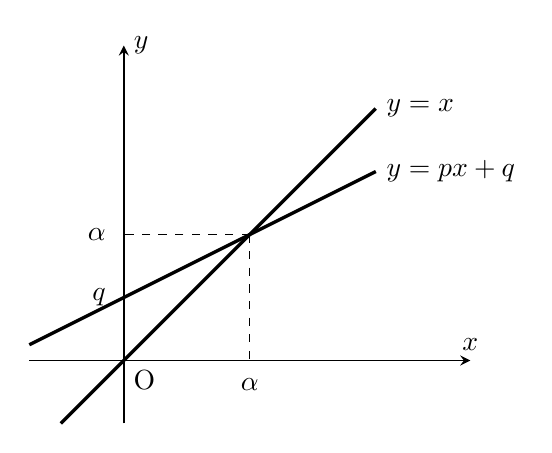
\begin{tikzpicture}[scale=0.8]
    \draw[->,>=stealth,semithick] (-1.5,0)--(5.5,0)node[above]{$x$};
    \draw[->,>=stealth,semithick] (0,-1)--(0,5)node[right]{$y$};
    \draw (0,0)node[below right]{O};

    \draw[very thick,domain=-1:4]
      plot(\x,\x)node[right]{$y=x$};

    \draw[very thick,domain=-1.5:4]
      plot(\x,\x/2+1) node[right] {$y=px+q$};

    % q
    \node[left=3pt] at (0,1) {$q$};

    % 交点から各軸へ点線
    \draw[dashed] (2,2) -- (2,0);
    \draw[dashed] (2,2) -- (0,2);

    % α
    \node[below=3pt] at (2,0) {$\alpha$};
    \node[left=3pt] at (0,2) {$\alpha$};
  \end{tikzpicture}
  \begin{center}
    \BookFigureCaption{直線の交点として捉える\bookterm{fixed}{不動点}}
  \end{center}

  というような状況である.
  この交点$(\alpha,\alpha)$を原点と思ってグラフをみると,この座標平面は$y=px$と$y=x$のグラフが原点から始まって進んでいくようなものに見える.
  言い換えれば等比型\bookterm{recurrence}{漸化式}に帰着させたということである.
  この交点の$x$座標$\alpha$が,更新$f$の\bookterm{fixed}{不動点}である.

  この\bookterm{fixed}{不動点}を知ることによって,複雑な値の変化をより簡素な値の変化に置き換えることができる.
  また,この話から,\,$|p|>1$のときは一般に項数を重ねるにつれて$p$が生み出す等比的な増大が支配的になる一方,\,$|p|<1$のときは$a_n$は$n\to\infty$で$\alpha=\dfrac{q}{1-p}$に収束し,その\bookterm{limit}{極限}値は$q$(と$p$)によって決まることが分かる.例題(2)(\,$p=\frac12$)が$4$に収束するのはこのためである.

  また,\bookterm{characteristic}{特性方程式}型\bookterm{recurrence}{漸化式}には別の解法が存在する.
  以下に示す.
  \begin{align*}
    &a_{n+1}=pa_n+q \tag*{\(\cdots\) (1)}\\
    &a_{n+2}=pa_{n+1}+q \tag*{\(\cdots\) (2)}\\
  \end{align*}
  $(2)-(1)$をし
  \[
    a_{n+2}-a_{n+1}=p(a_{n+1}-a_n)
  \]
  ここで,\,$b_n=a_{n+1}-a_n$と置くと,
  \begin{align*}
    &b_{n+1}=pb_n
  \end{align*}
  このようにすることで,\bookterm{recurrence}{漸化式}は\bookterm{geometric}{等比数列}に帰着する.
  得られた差を初項から足し戻すと、元の\bookterm{sequence}{数列}が求まる。

  こちらの図形的解釈は先程の交点を考えるものとは違う.傾き$p$の平行な2直線$y=px$と$y=px+q$の間には,常に高さ$q$の差が生じている.\,(2)から(1)を引く操作は,この共通の$q$だけを打ち消す操作に対応している.つまり隣接する2つの式を「ずらして引く」ことで,\,$a_n$に無関係な定数項$q$だけを消してしまうのである.これは付録\sectionref{節：差分から始まる離散的な微積分}で扱う\bookterm{difference-operator}{差分}の考え方と同じ発想である.
  これらの前提を元に図示すると

  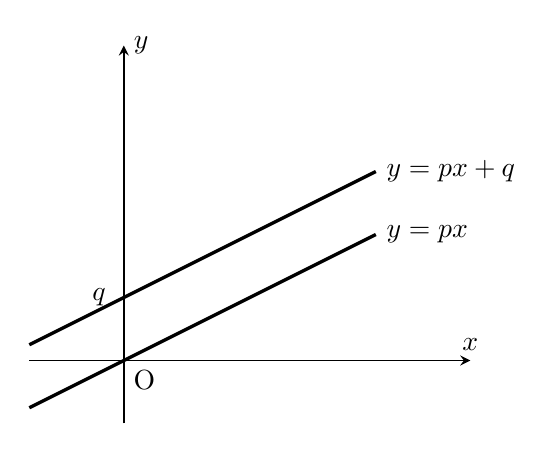
\begin{tikzpicture}[scale=0.8]
    \draw[->,>=stealth,semithick] (-1.5,0)--(5.5,0)node[above]{$x$};
    \draw[->,>=stealth,semithick] (0,-1)--(0,5)node[right]{$y$};
    \draw (0,0)node[below right]{O};

    \draw[very thick,domain=-1.5:4]
      plot(\x,\x/2)node[right]{$y=px$};

    \draw[very thick,domain=-1.5:4]
      plot(\x,\x/2+1) node[right] {$y=px+q$};

    % q
    \node[left=3pt] at (0,1) {$q$};

  \end{tikzpicture}
  \begin{center}
    \BookFigureCaption{定数項の違いを表す平行な直線}
  \end{center}

  常に関数の差が$q$と一定になっていることが図からわかる.

  なお,先ほどの等比的な増大について,初項を\bookterm{fixed}{不動点}に選んだ場合は例外になる.
  \bookterm{fixed}{不動点}から出発すれば値は変わらず,\,$a_n=\alpha$という定\bookterm{sequence}{数列}になるからである.
  式で確かめると,\,$p\ne1$のときは
  \[
    a_n-\alpha=(a_1-\alpha)p^{n-1}
  \]
  である.したがって,\,$|p|>1$でも$a_1=\alpha$ならずれは常に$0$であり,\,$a_1\ne\alpha$の場合に\bookterm{fixed}{不動点}からのずれの絶対値が等比的に増大する.

  今後,\bookterm{characteristic}{特性方程式}を用いた解法を多数扱う.
  \bookterm{characteristic}{特性方程式}は\bookterm{recurrence}{漸化式}を解く中で重要な概念なのである.
  その背景には\bookterm{matrix}{行列}や\bookterm{linear}{線形}代数が深く絡んでいる.
